\section{Functions}
\textbf{Definition} A function is a correspondence between input numbers(x-values) and output numbers(y-values) such that each input number is paired with exactly one output number. \\
A non-mathematical example of a function is a vending machine. The input is the money(x-values) you put in and the output is the item you get(y-values). You can't put in the same amount of money and get two different items. \\

Functions can be described with an equation.

\textbf{Example}. $y = x^2 + 1$, which can also be written as $f(x) = x^2 + 1$. \\
\vspace{4pt}

What is $f(2)$ ? $ f(5) ?$ \\
\vspace{4pt}

In mathematics, the notation "f(x)" is commonly used to represent a function. In this notation, "f" is the name of the function, and "x" is the input or independent variable. When you write "f(x)," you are essentially saying "the value of the function f when the input is x."

The function itself is a rule or relationship that assigns a unique output (often denoted as "y") for each input value "x." So, when you evaluate "f(x)," you are finding the corresponding output value for the given input. (VIDEO HERE)

Here's a simple example to illustrate this:

Let's say you have a function defined as:
f(x) = 2x + 3

If you want to find the value of the function when x is 4, you would write it as:
$f(4) = 2 \cdot 4 + 3 = 8 + 3 = 11$

So, in this case, f(4) refers to the y-value or the output of the function when x is 4, and it equals 11. The notation "f(x)" is just a way to represent this relationship between inputs (x-values) and outputs (y-values) in a concise and standardized manner.

When we write $f(2)$, we are asking what is the value of the function when $x = 2$. 
So we take $2$ and plug it in for $x$ in the equation. \\

$$f(2) = 2^2 + 1 = 5$$
$$f(5) = 5^2 + 1 = 26$$ \\

Similarly, we can ask what is $f(a + 3)$
$$ f(a + 3) = (a+3)^2 + 1 = a^2 + 6a + 10 $$
\vspace{4pt}

We can also describe a function with a graph. \\
\textbf{Example}. The graph if $y = g(x)$ is shown below
\begin{align*}
	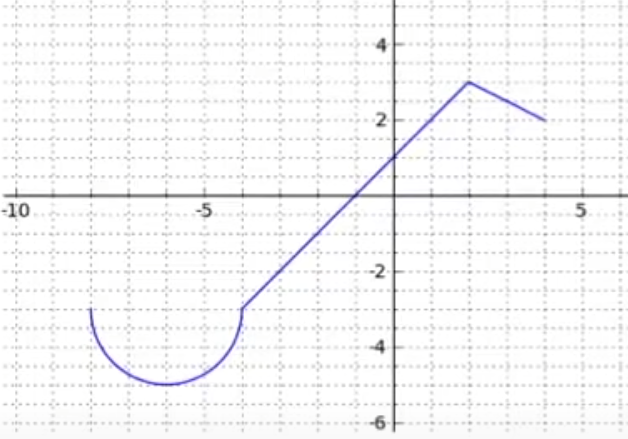
\includegraphics{algebra-pre-calculus/functions/graph1.png}
\end{align*}
\vspace{1pt}
What is $g(2)$ ? $ g(5) ?$ \\

First let's establish that $ y = g(x) $ so they are essentially mean the same thing. \\
In mathematics, when we write "$g(x)=y$," we are essentially saying that the value of the function $g$ when given the input $x$ is equal to the value $y$. This relationship is expressed as:
$$ g(x) = y $$
Here's what each part of this notation means: 
\begin{itemize}
	\item $g(x)$ represents the output or value of the function $g$ when you input the value $x$.
	\item "=" denotes equality, indicating that the output of $g(x)$ is equal to $y$.
\end{itemize}


In $g(2)$, $2$ corresponds to the $x$-value that is passed through the function and we will use the graph to find corresponding $y$-value. \\
Since we know that we have to look for the $x$-value of $2$, we can look at the graph and find the point where $x = 2$. \\
Then we can look at the $y$-value of that point and that will be $3$. \\
Therefore, $g(2) = 3$. \\
Now when we look at $g(5)$, we can use the same method. However, we run into an issue that when we look at the x-value of $5$, we see that there is no point on the graph that has that x-value. \\
Therefore, $g(5)$ is undefined. \\
The question of what x-values and y-values makes sense to a function leads to the \textbf{domain} and \textbf{range} for a function. \\

\subsection{Domain and Range of a Function}
\textbf{Domain}: The domain of a function is the set of all possible x-values. \\
\textbf{Range}: The range of a function is the set of all possible y-values. \\

Let's examine the graph again and determine its range and domain. To find the domain of a function we have to look at the x-values that corresponds a point on the graph. \\
\begin{align*}
	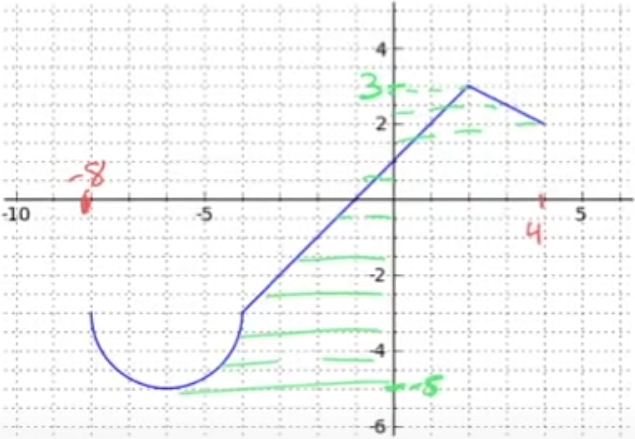
\includegraphics{algebra-pre-calculus/functions/graph2.png}
\end{align*}

We can see that the \textbf{domain} is $-8 \le x \le 4$. \\
Or as an interval notation, $[-8, 4]$. \\

To find the range of a function we have to look at the y-values that corresponds a point on the graph. \\
\textbf{range} is $-5 \le y \le 3$. \\
Or as an interval notation, $[-5, 3]$. \\

\subsection{Domain and Range of a Function as an Equation}
\textbf{Example}. Find the domain of these functions. \\
$\displaystyle A. \ g(x) = \frac{x}{x^2 - 4x + 3}$ \\
$\displaystyle B. \ f(x) = \sqrt{3-2x}$ \\
To find the domain of a function we have to consider algebraic restrictions. We can go ahead and question what values make sense to plug in for $x$. \\
Therefore,
\begin{itemize}
	\item 1. Exclude x-values that make the denominator 0.
	\item 2. Exclude x-values that make the radicand(number under the radical) negative. Since we cannot take the square root of a negative number.
\end{itemize}

What we have to do in the first function is this:
\begin{align*}
	x^2-4x+3 & \neq 0 \quad \text{Since the denominator cannot be 0} \\
\end{align*}

In other words we can solve the equation to be equal to 0 and exclude its solutions
\begin{align*}
	x^2-4x+3   & = 0 \quad \text{Factorise the quadratic} \\
	(x-3)(x-1) & = 0                                      \\
	x          & = 3, 1                                   \\
\end{align*}
Therefore we need to exclude $x=3$ and $x=1$ from the domain. \\

We can represent the domain as an interval notation. \\
\textbf{Domain} is $(-\infty, 1) \cup (1, 3) \cup (3, \infty)$. \\
Meaning that the domain is all real numbers except $1$ and $3$. \\

Now let's look at the second function.

Since we cannot take the square root of a negative number, we have to make sure that the radicand is not negative. \\

Therefore, we exclude the numbers:
$$ 3-2x < 0$$

Similarly we can include everyone number that makes the radicand positive(bigger than zero). \\
$$ 3-2x \ge 0$$
$$ 3 \ge 2x$$
$$ \frac{3}{2} \ge x$$

Therefore, the domain is $(-\infty, \frac{3}{2}]$.
Notice that we used a square bracket instead of a round bracket. This is because we can include the number $\frac{3}{2}$ in the domain. \\

\subsection{Function as a fractional equation with radicals}

\textbf{Example}. $\displaystyle h(x)=\frac{\sqrt{3-2x}}{x^2-4x+3}$ \\

So we have to consider the same restrictions as before. \\

\begin{align*}
	x^2-4x+3 &\neq 0 \quad \text{Since the denominator cannot be 0} \\
	3-2x &\ge 0 \quad \text{Since we cannot take the square root of a negative number} \\
\end{align*}

We've already solved the first condition which was $x\neq3$ and $x\neq1$. \\
The second condition is $x\le\frac{3}{2}$. \\

Therefore our domain is $(-\infty, 1) \cup (1, \frac{3}{2}]$.

\subsection{Increasing and Decreasing Functions}

\textbf{Example.} Which function is Increasing and which is Decreasing?

\begin{align*}
	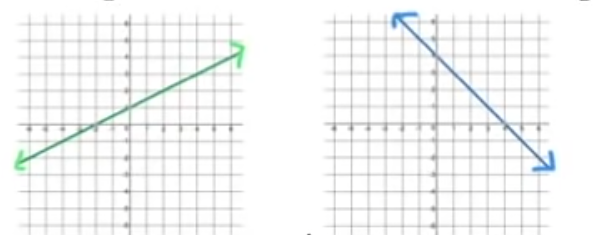
\includegraphics{algebra-pre-calculus/functions/graph3.png}
\end{align*}

As seen the first function is increasing and the second function is decreasing. 

This can be written more formaly as: \\
$ x_1 < x_2 \Rightarrow f(x_1) < f(x_2) $ \\
$x_1$ and $x_2$ are two arbitrary x-values. \\
This means that the y-values are increasing as the x-values are increasing. \\

In the decreasing function, the y-values are decreasing as the x-values are increasing. 
$ x_1 < x_2 \Rightarrow f(x_1) > f(x_2) $ \\

\textbf{Example.} On what intervals is the function graphed below increasing? Decreasing? 
\begin{align*}
	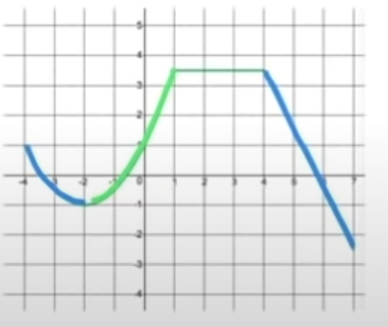
\includegraphics{algebra-pre-calculus/functions/graph4.png}
\end{align*}

We are going to solve this in terms of the x-values. Simply because the y-values can be same for different parts of the graph but the x-values are unique.
\textbf{Decreasing}: $-4\le x<-2, \quad 4<x\le7 $ \\
\textbf{Increasing}: $-2< x<1$ \\
As intervals: $[-4, -2) \cup (4,7), (-2, 1)$ \\

\subsection{Maximums and Minimums on Graphs}
\textbf{Definition.} An absolute maximum of a function, also known as a global maximum, is the highest value that the function can attain over its entire domain. In other words, it is the largest output (or y-value) that the function can produce for any input (or x-value) within its defined domain. \\
In other words a function f(x) has an absolute maximum at $x = c$ if $f(c) \ge f(x)$ for all $x$ in the domain of $f$. \\
The y-value f(c) is called the absolute maximum value of $f$. \\
and the point $(c, f(c))$ is called the absolute maximum point of $f$. \\

\begin{align*}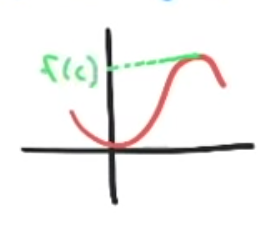
\includegraphics{algebra-pre-calculus/functions/graph5.png}\end{align*}
Here we can see that essentially the absolute maximum is the highest point on the graph. \\
And the absolute value point would be the point where it achieves the absolute maximum. \\
A function can have multiple absolute maximum points(multiple points referencing to the absolute maximum of the function), however it can only have one absolute maximum value. \\

\textbf{Definition}. The absolute minimum of a function, also known as a global minimum, is the lowest value that the function can attain over its entire domain. In other words, it is the smallest output (or y-value) that the function can produce for any input (or x-value) within its defined domain. \\
The absolute minimum of a function $f(x)$ is the smallest value of $f(x)$ over its entire domain. \\
In other words a function f(x) has an absolute minimum at $x = c$ if $f(c) \le f(x)$ for all $x$ in the domain of $f$. \\
The y-value f(c) is called the absolute minimum value of $f$. \\
and the point $(c, f(c))$ is called the absolute minimum point of $f$. \\

\begin{align*}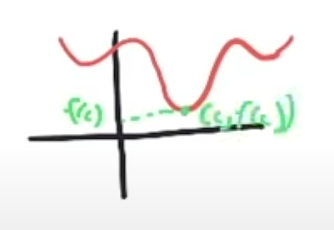
\includegraphics{algebra-pre-calculus/functions/graph6.png}\end{align*}
Here we can see that essentially the absolute minimum is the lowest point on the graph. \\
And the absolute value point would be the point where it achieves the absolute minimum. \\
A function can have multiple absolute minimum points(multiple points referencing to the absolute minimum of the function), however it can only have one absolute minimum value. \\
\newpage
\subsection{Local Maximums and Minimums}
\textbf{Definition.} A local maximum of a function is a point on the graph where the y-value is greater than or equal to all the y-values of points in the nearby region. \\
A function f(x) has a local maximum at $x = c$ if $f(c) \ge f(x)$ for all $x$ in some open interval around $c$. \\

In other words, the way we identify local maximums is by looking at the graph and seeing if there is a point where an interval around that point exists such that all function values within that interval are less than or equal to the function value at that specific point. If this condition is met, we can conclude that the function has a local maximum at that point.

A local minimum of a function is a point on the graph where the y-value is less than or equal to all the y-values of points in the nearby region. \\
A function f(x) has a local minimum at $x = c$ if $f(c) \le f(x)$ for all $x$ in some open interval around $c$. \\
In other words, the way we identify local minimums is by looking at the graph and seeing if there is a point where an interval around that point exists such that all function values within that interval are greater than or equal to the function value at that specific point. If this condition is met, we can conclude that the function has a local minimum at that point. \\

\textbf{Definition}. Local maximum and minimum points are also called relative maximum and minimum points. \\
\textbf{Definition}. A point where a function changes from increasing to decreasing or decreasing to increasing is called a turning point. \\

\newpage
\begin{figure}
	\centering
	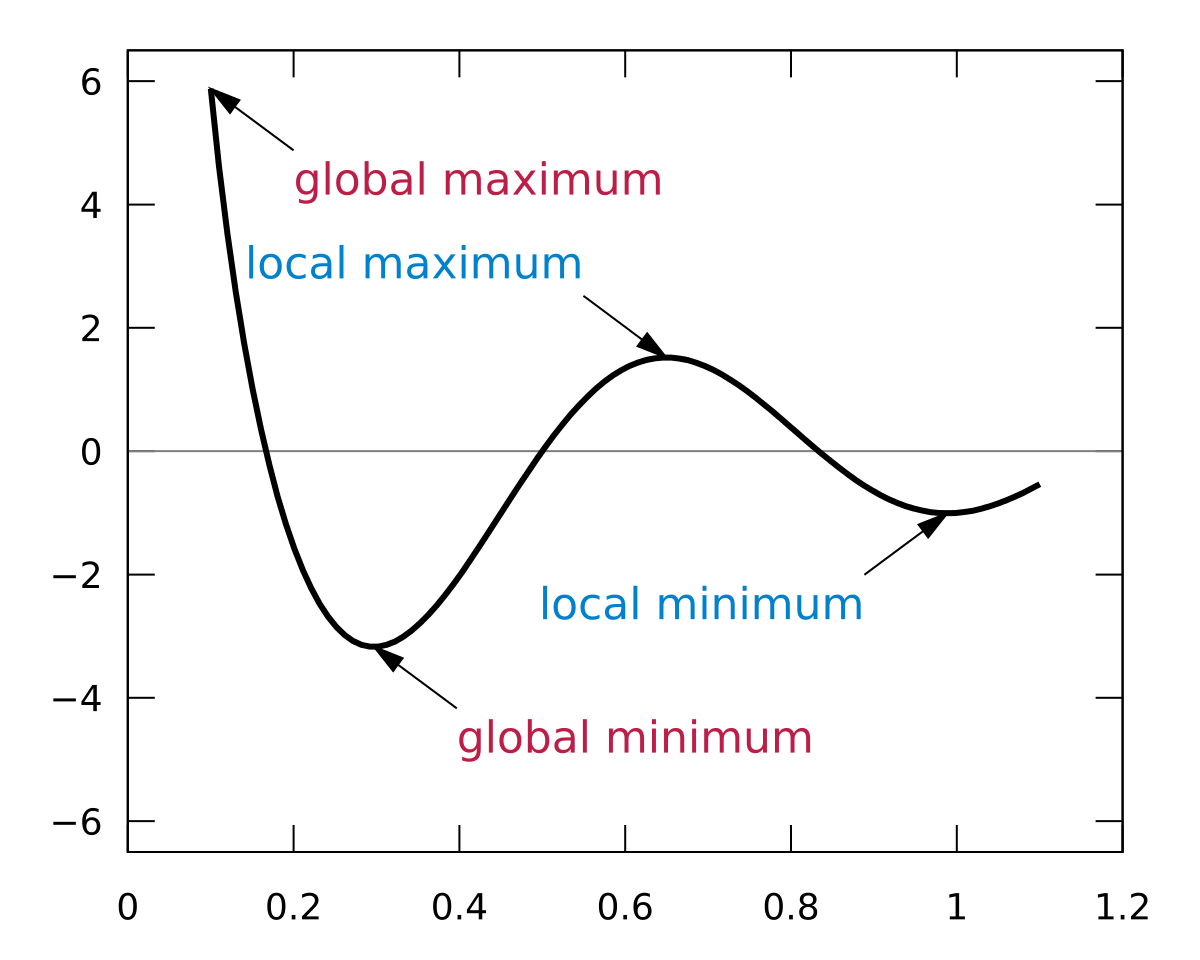
\includegraphics[width=0.5\textwidth]{algebra-pre-calculus/functions/graph7.png}
	\caption{Absolute Maximum and Minimum with Local Maximum and Minimum}
\end{figure}

\subsection{Example}


\begin{align*}
	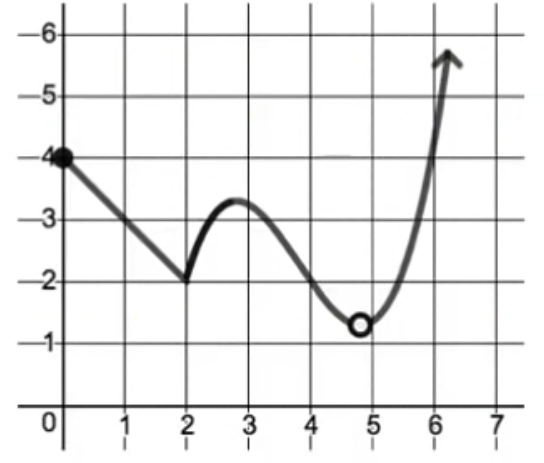
\includegraphics{algebra-pre-calculus/functions/example_graph.png}
\end{align*}

\textbf{Example.} 
\begin{enumerate}
	\item Mark all local maximum and minimum points on the graph. 
	\item Mark all absolute maximum and minimum points on the graph.
	\item What are the local maximum and minimum values?
	\item What are the absolute maximum and minimum values?
\end{enumerate}

\textbf{Solution.} \\
The function has a local maximum point here: $(2.7,-3.3)$ \\
There is a local minimum point here: $(2, 2)$ \\
The point with the drilled out circle means that it is not part of the graph. If it would be then that point would be a local minimum point and an absolute minimum point. \\ 
The point $(0,4)$ by some sources considered to be a local maximum point, However by other sources it doesn't. 
Therefore, we do not have any absolute maximum points, as the arrow indicates that the function goes to infinity. \\
We don't have any absolute minimum points either. \\
Now for talking about the values, we can see that the local maximum value is $-3.3$ and the local minimum value is $2$ which are just the y-values of the points. \\
We do not have any absolute maximum or minimum values.

\subsection{Even and Odd Functions Part 1}
\textbf{Definition.} A graph is symmetric with respect to the x-axis if whenever $(x,y)$ is on the graph, then $(x,-y)$(its mirror point) is also on the graph, and it has mirror symmetry across the x-axis as the mirror line. \\
\begin{align*}
	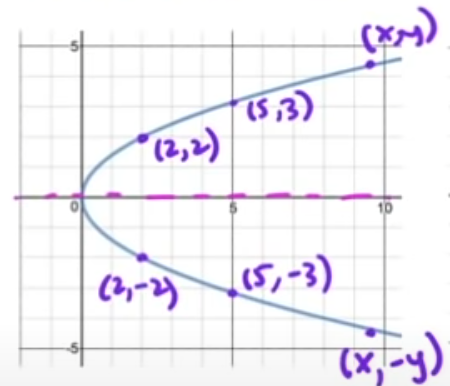
\includegraphics{algebra-pre-calculus/functions/even_odd_graph1.png} \\
\end{align*}

As you can see the graph is symmetric since if we take a point, then the point with the same x-value but with a negative y-value is also on the graph. \\
\textbf{Definition.} A graph is symmetric with respect to the y-axis if whenever $(x,y)$ is on the graph, then $(-x,y)$(its mirror point) is also on the graph, and it has mirror symmetry across the y-axis as the mirror line. \\

\begin{align*}
	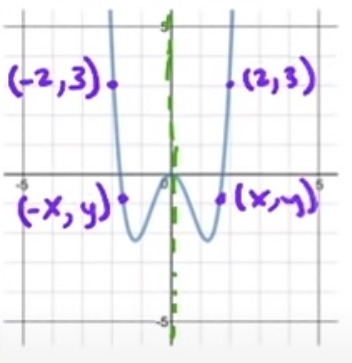
\includegraphics{algebra-pre-calculus/functions/even_odd_graph2.png} \\
\end{align*}

As you can see the graph is symmetric since if we take a point, then the point with the same y-value but with a negative x-value is also on the graph. \\
\textbf{Definition.} A graph is symmetric with respect to the origin if it has 180 degree rotational symmetry around the origin. \\
In other words if we rotate the graph 180 degrees around the origin, then the graph will be the same. \\

\begin{align*}
	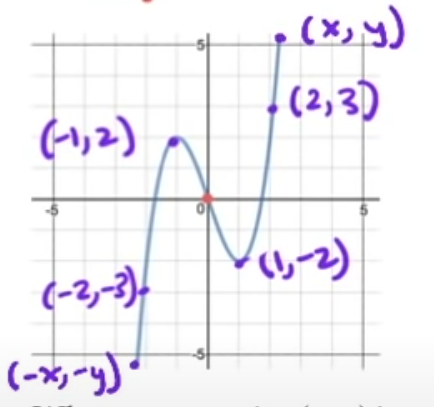
\includegraphics{algebra-pre-calculus/functions/even_odd_graph3.png} \\
\end{align*}
As you can see the origin is the center of the graph and if we rotate the graph 180 degrees around the origin, then the graph will be the same. \\
In terms of the points if we want to find the mirror point of $(x,y)$, then we have to take the negative(opposite, so if it's negative then it should turn to positive) of both the x and y values which is $(-x,-y)$. \\

\subsection{Examples to identify symmetry}

\textbf{Example.} Which graphs are symmetric with respect to the x-axis, the y-axios, the origin or neither? \\

\begin{align*}
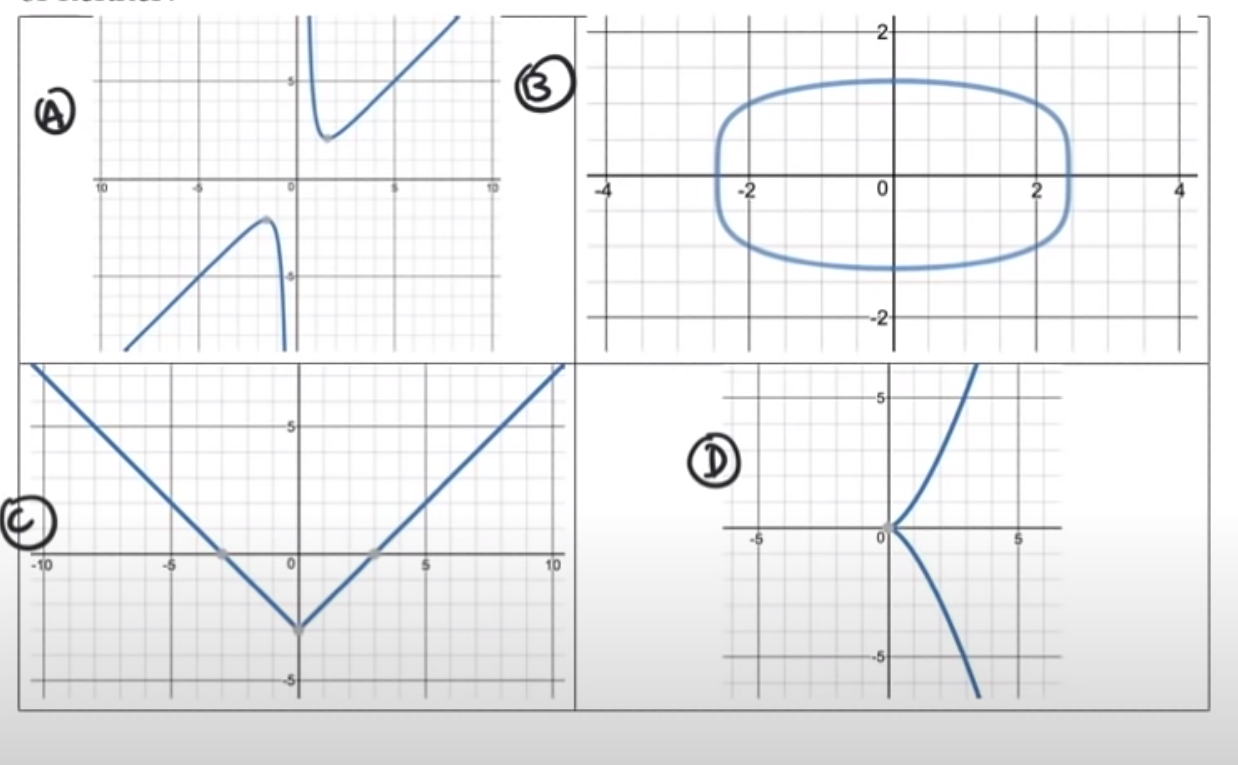
\includegraphics[width=1.2\textwidth]{algebra-pre-calculus/functions/even_odd_example1.png}
\end{align*}

\textbf{Solution.} \\
A. Symmetric with respect to the origin since if we rotate the graph 180 degrees around the origin, then the graph will be the same. \\
B. Symmetric with respect to the y-axis, x-axis, and origin. \\
C. Symmetric with respect to the y-axis. \\
D. Symmetric with respect to the x-axis. \\


\subsection{Even and Odd Functions Part 2}

\textbf{Definition.} A function $f(x)$ is even if its graph is symmetric with respect to the y-axis. Meaning that whenever $(x,y)$ is on the graph, then $(-x,y)$(its mirror image) is also on the graph. \\
That is the y-values corresponding to the $x$ and $-x$ are the same. \\
Since $y = f(x)$ we can say that the points are $(x,f(x))$ and $(-x,f(-x))$. \\
In conclusion  we can say that $f(x) = f(-x)$ for all x-values in its domain. Since they are representing the y-values which are the same. 
see here: 
\begin{align*}
	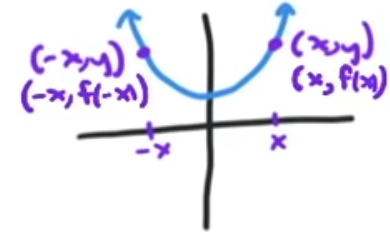
\includegraphics{algebra-pre-calculus/functions/even_odd_example2.png} \\
\end{align*}

\textbf{Example.} $f(x) = x^2+3$ is an even function because... \\
\textbf{Solution.} $f(-x) = (-x)^2+3 = x^2+3 = f(x)$ \\

\textbf{Definition.} A function $f(x)$ is odd if its graph is symmetric with respect to the origin. Meaning that whenever $(x,y)$ is on the graph, then $(-x,-y)$(its mirror image) is also on the graph. \\
The graphs y-value at x and the graphs y-value at -x are the opposites of each other. \\
Since $y = f(x)$ we can say that the points are $(x,f(x))$ and $(-x,-f(-x))$. \\
In conclusion  we can say that $f(-x) = -f(x)$ for all x-values in its domain. This means that the y-values are the opposites of each other. \\
see here:
\begin{align*}
	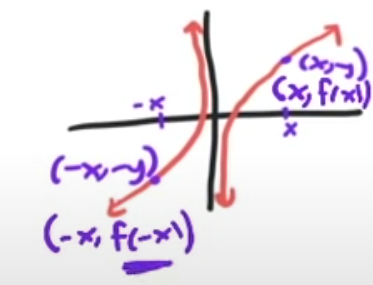
\includegraphics{algebra-pre-calculus/functions/even_odd_example3.png} \\
\end{align*}
\textbf{Example.} $f(x) = 5x-\frac{1}{x}$ is an odd function because... \\
\textbf{Solution.} $f(-x) = 5(-x)-\frac{1}{-x} = -5x+\frac{1}{x} = -(5x-\frac{1}{x}) = -f(x)$ \\

In conclusion we covered that functions that are symmetric with respect to the y-axis are even functions and functions that are symmetric with respect to the origin are odd functions. \\
The reason why we haven't covered functions that are symmetric with respect to the x-axis is because they are neither even nor odd and more importantly they are NOT functions which we will touch on later. \\

\subsection{Toolkit Functions}
Let's look at some toolkit functions.
\begin{align*}
	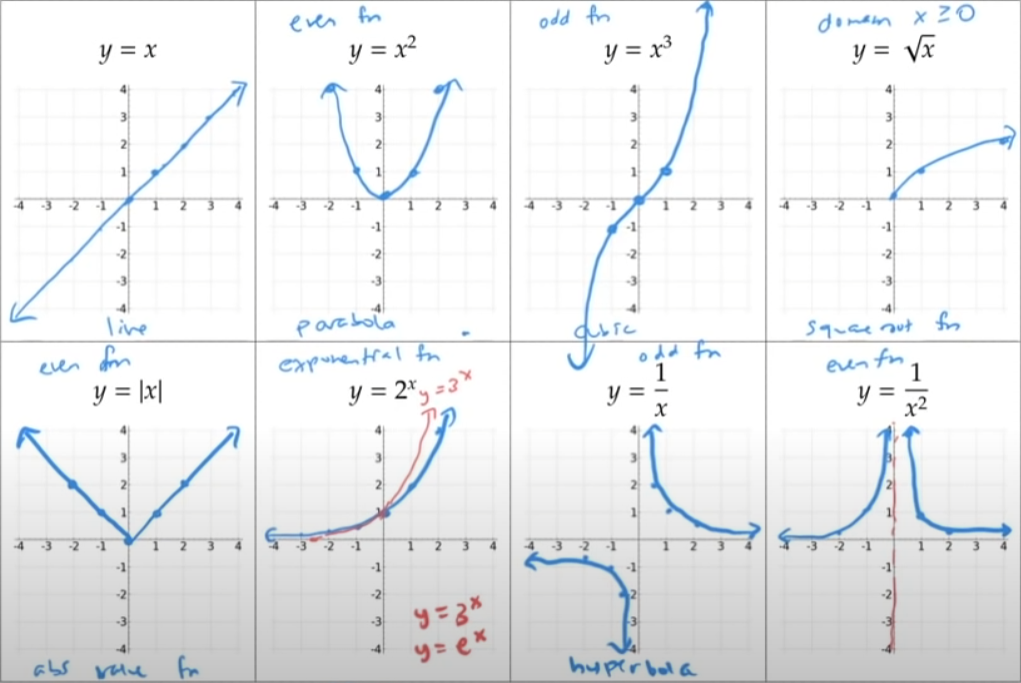
\includegraphics[width=1.1\textwidth]{algebra-pre-calculus/functions/toolkit_functions.png}
\end{align*}

Let's go through each of them and explain what they are and how do they work.

\begin{enumerate}
	\item First function is $y=x$ which is a linear function. It is a straight line that goes through the origin. When $x=0$, $y=0$. When $x=1$, $y=1$. When $x=-1$, $y=-1$. When $x=2$, $y=2$. When $x=-2$, $y=-2$. And so on. 
	\item Second function is $y=x^2$ which is a quadratic function. It is a parabola that goes through the origin. When $x=0$, $y=0$. When $x=1$, $y=1$. When $x=-1$, $y=1$. When $x=2$, $y=4$. When $x=-2$, $y=4$. And so on. Also notice that this function is an even function with respect to the y-axis. The left-side of the graph is the mirror image of the right-side of the graph. This happens is because if you square a negative number, then you get a positive number.
	\item Third function is $y=x^3$ which is a cubic function. It is a cubic function that goes through the origin. When $x=0$, $y=0$. When $x=1$, $y=1$. When $x=-1$, $y=-1$. When $x=2$, $y=8$. When $x=-2$, $y=-8$. And so on. Also notice that this function is an odd function with respect to the origin. The bottom-side of the graph is the mirror image of the top-side of the graph. This happens is because if you cube a negative number, then you get a negative number and so on.
	\item Fourth function is $y=\sqrt{x}$ which is a square root function. It is a function that starts at the origin and goes up. When $x=0$, $y=0$. When $x=1$, $y=1$. When $x=4$, $y=2$. When $x=9$, $y=3$. And so on. Notice that this function is not defined for negative numbers. This is because we cannot take the square root of a negative number. Also notice that this function is not an even or odd function. This is because the graph is not symmetric with respect to the y-axis or the origin.
	\item Fifth function is $y=|x|$ which is an absolute value function. It is a function that starts at the origin and goes up. When $x=0$, $y=0$. When $x=1$, $y=1$. When $x=-1$, $y=1$. When $x=2$, $y=2$. When $x=-2$, $y=2$. And so on. Notice that the function doesn't have a negative y-value. This is because the absolute value of a number is always positive. Also notice that this function is an even function with respect to the y-axis. The left-side of the graph is the mirror image of the right-side of the graph. This happens is because if you take the absolute value of a negative number, then you get a positive number.
	\item Sixth function is $y=2^x$ which is an exponential function. This looks like an exponential growth. Everytime we increase the x by 1, the y-value doubles. Also notice that this function is not an even or odd function. This is because the graph is not symmetric with respect to the y-axis or the origin. If we increase the base from 2 to 3, then the graph will look like an exponential growth but steeper.
	\item Seventh function is $y=\frac{1}{x}$ which is a reciprocal function. This looks like a hyperbola. When $x=1$, $y=1$. When $x=2$, $y=\frac{1}{2}$. When $x=3$, $y=\frac{1}{3}$. When $x=4$, $y=\frac{1}{4}$. And so on. Notice that this function is not defined for $x=0$. This is because we cannot divide by zero. Also notice that this function is an odd function with respect to the origin. The bottom-side of the graph is the mirror image of the top-side of the graph. 
	\item  Eighth function is $y=\frac{1}{x^2}$ which is a reciprocal squared function. This looks like a hyperbola. When $x=1$, $y=1$. When $x=2$, $y=\frac{1}{4}$. When $x=3$, $y=\frac{1}{9}$. When $x=4$, $y=\frac{1}{16}$. And so on. Notice that this function is not defined for $x=0$. This is because we cannot divide by zero. Also notice that this function is an even function with respect to the y-axis. The left-side of the graph is the mirror image of the right-side of the graph. 
\end{enumerate}

\subsection{Review of Function Notation}
\textbf{Review of Function Notation.} \\
The expression $g(x) = \sqrt{x}$ defines a function called g. In this function:

\begin{itemize}
	\item $g(x)$ represents the output or value of the function when you input the value $x$.
	\item $\sqrt{x}$ denotes the square root of the input $x$.
\end{itemize}
So, this function $g$ takes an input value $x$ and returns its square root as the output. In other words, for any real number $x$ in the domain of this function where $\sqrt{x}$ is defined (which is typically for non-negative real numbers or zero as you cannot square root a negative number), $g(x)$ will be equal to the square root of $x$. Because we took the input $x$ and plugged it into the function $g$, and following the function's rule, we took the square root of $x$ to get the output value $g(x)$ which is what the functions "returns". We can think of mathematical functions as functions in programming, since there we have a function that defines and executes a set of instructions and returns a value. In this case, the function $g$ takes an input $x$(parameter) and returns the square root of $x$ as the output $g(x)$, therefore we can say that functions in programming are similar to mathematical functions significantly. \\

For example, if you plug in $x = 4$ into this function, you would get:

$g(4) = \sqrt{4} = 2$

So, when $x$ is 4, $g(x)$ is 2. This function represents a basic mathematical operation that calculates the square root of its input.

\textbf{Example.} Rewrite the following, if $g(x) = \sqrt{x}$ \\
What we do is plug in the value of $x$ into the function $g$ and then we execute the function's "body" using that $x$ parameter. \\
\begin{enumerate}
	\item [(a)] $g(x)-2=\sqrt{x}-2 \quad \text{Since $g(x)=\sqrt{x}$}$
	\item [(b)] $g(x-2) = \sqrt{x-2}$ \quad
	We just replaced $x$ with $x-2$ as that is the input("parameter") to our function $g$.
	\item [(c)] $g(3x) = \sqrt{3x}$ \quad
	\item [(d)] $3g(x) = 3(\sqrt{x})$ \quad \text{Since $g(x)=\sqrt{x}$}
	\item [(e)] $g(-x) = \sqrt{-x}$ \quad
	This might look odd since we cannot take the square root of a negative number. However, remember that if $x$ is negative, then $-(-x)$ is positive. Therefore, we can take the square root of $-x$ in that case.
\end{enumerate}

Now let's do the opposite.
\textbf{Example.} Rewrite the following in terms of g(x), if $g(x) = \sqrt{x}$ \\
\begin{enumerate}
	\item [(f)] $\sqrt{x}+17=g(x)+17$
	\item [(g)] $\sqrt{x+12}=g(x+12)$ \quad Since $\sqrt{x}=g(x)$ and $x+12$ is the input to the function $g$. Therefore, $\sqrt{x+12}=g(x+12)$ Because we can put anything to the function's input("paramater").
	\item [(h)] $-36\cdot\sqrt{x}=-36\cdot g(x)$
	\item [(i)] $\sqrt{\frac{1}{4}x}=g(\frac{1}{4}x)$ \quad Again whatever we put into the function's input("parameter") is going to be square rooted. Because $g(x)=\sqrt{x} \quad \Rightarrow \quad g(anything)=\sqrt{anything}$
\end{enumerate}

\subsection{Graphing Functions}
if we have an example function $g(x) = \sqrt{x}$, then we can graph it by plugging in all of the values from the x-axis as inputs("parameters") for $x$ and then plotting the corresponding $y$-values and seeing that which x-value corresponds to which y-value. \\
\textbf{Example.} Graph the functions: \\
\begin{enumerate}
	\item $y=\sqrt{x}$ This means that every x value along the x-axis is going to be square rooted and that will be its corresponding y-value. \\
	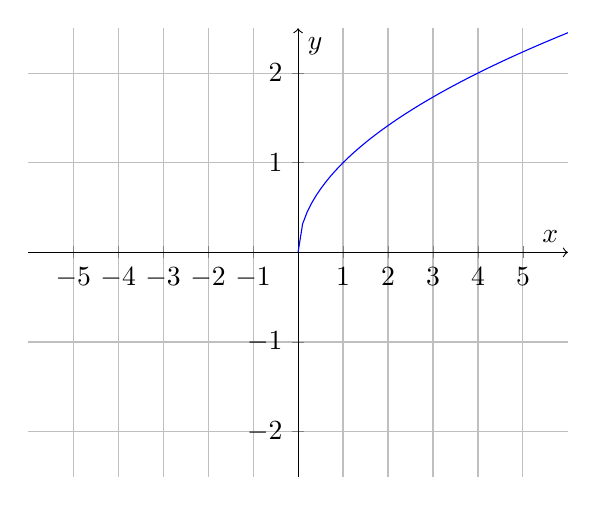
\begin{tikzpicture}
		\begin{axis}[
			xlabel={$x$},
			ylabel={$y$},
			axis lines=middle,
			axis line style={->},
			xmin=-6,
			ymin=-2.5,
			xmax=6,
			ymax=2.5,
			xtick={-5,-4,-3,-2,-1,0,1,2,3,4,5},
			ytick={-2,-1,0,1,2},
			legend style={at={(0.95,0.95)},anchor=north east},
			grid=both
		  ]
			\addplot[domain=0:10, samples=100, color=blue]{sqrt(x)};
		  \end{axis}
		\end{tikzpicture} \\
		We are going through every x-value and square rooting it and that will give its corresponding y-value.
		So for example when $x=4$, $y=\sqrt{4}=2$. When $x=9$, $y=\sqrt{9}=3$. When $x=16$, $y=\sqrt{16}=4$. And so on. \\  
		\item $y=\sqrt{x}-2$ This means that every x value along the x-axis is going to be square rooted and then subtracted by 2 and that will be its corresponding y-value. \\
		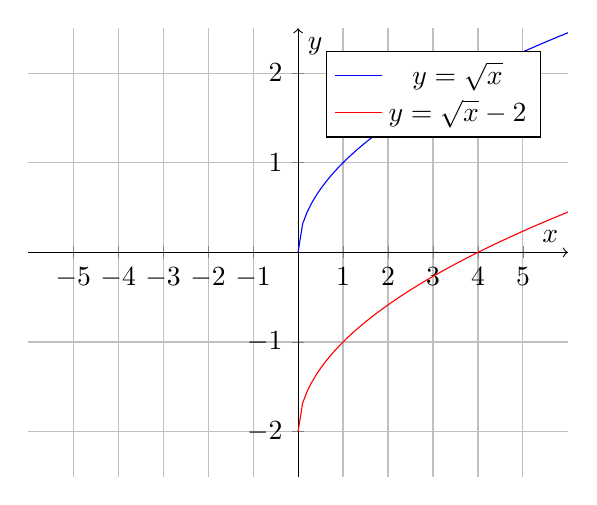
\begin{tikzpicture}
			\begin{axis}[
			  xlabel={$x$},
			  ylabel={$y$},
			  axis lines=middle,
			  axis line style={->},
			  xmin=-6,
			  ymin=-2.5,
			  xmax=6,
			  ymax=2.5,
			  xtick={-5,-4,-3,-2,-1,0,1,2,3,4,5},
			  ytick={-2,-1,0,1,2},
			  legend style={at={(0.95,0.95)},anchor=north east},
			  grid=both
			]
			  \addplot[domain=0:10, samples=100, color=blue]{sqrt(x)};
			  \addlegendentry{$y=\sqrt{x}$} % Add a legend entry for the first plot
			  % Add a new plot here:
			  \addplot[domain=0:10, samples=100, color=red]{sqrt(x)-2};
			  \addlegendentry{$y=\sqrt{x}-2$} % Add a legend entry for the second plot
			\end{axis}
		  \end{tikzpicture}		 
		  Because we subtracted 2 outside of the square root, the graph is shifted down by 2.
		  \item $y=\sqrt{x-2}$ This means that every x value along the x-axis is going to be subtracted by 2 and then square rooted and that will be its corresponding y-value. \\
		  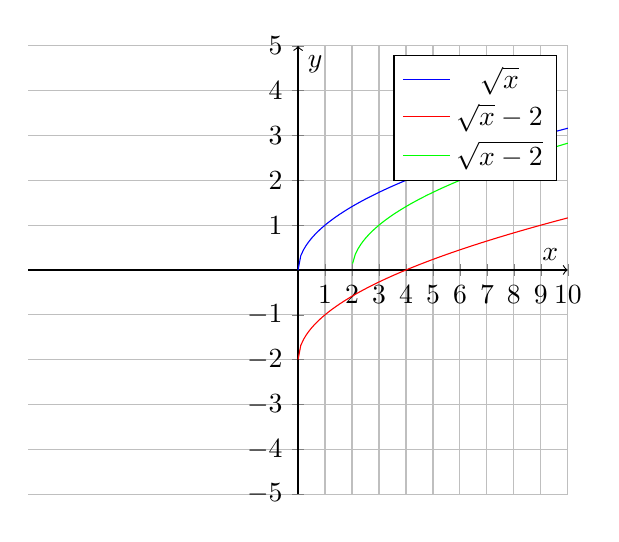
\begin{tikzpicture}
			\begin{axis}[
			  xlabel={$x$},
			  ylabel={$y$},
			  axis lines=middle,
			  axis line style={->},
			  xmin=-10,
			  ymin=-5,
			  xmax=10,
			  ymax=5,
			  xtick={0,1,2,3,4,5,6,7,8,9,10},
			  ytick={-5,-4,-3,-2,-1,0,1,2,3,4,5,6,7,8,9,10},
			  grid=both
			]
			  \addplot[domain=0:10, samples=100, color=blue]{sqrt(x)};
			  \addlegendentry{$\sqrt{x}$} % Add a legend entry for the first plot
			  % Add a new plot here:
			  \addplot[domain=0:10, samples=100, color=red]{sqrt(x)-2};
			  \addlegendentry{$\sqrt{x}-2$} % Add a legend entry for the second plot
			  \addplot[domain=0:10, samples=100, color=green]{sqrt(x-2)};
			  \addlegendentry{$\sqrt{x-2}$} % Add a legend entry for the second plot
			\end{axis}
		  \end{tikzpicture}	
		  As we can see the graph is shifted to the right by 2.  We might expect the graph to go left by 2 as we subtracted 2. However, the graph is shifted to the right by 2. \\
		  This is because when we are evaluating the function $y=\sqrt{x-2}$, What we are doing is goin through the x-axis and putting each of the x-values into the function and evaluate them by the function's rule. \\
		  So since we cannot square a negative number when $x=-1$ where the y-value would be $\sqrt{-1-2}=\sqrt{-3}$, we cannot evaluate the function. \\
		  As we go through these values we can see that the first value that we can evaluate the function is when $x=2$. \\
		  Because, $y=\sqrt{2-2}=\sqrt{0}=0$. \\
		  Since this is the first value that makes sense we can start the graph from 2. \\
		  That's why the function is being shifted by 2 to the right, because 2 is the first value that makes sense to the function or in other words this is the first value that mathematically can be evaluated. 
		  If we would have $y=\sqrt{x+2}$ then the graph would be shifted to the left by 2. Because the first value that makes sense to the function is -2. \\
\end{enumerate}

Let's look at some rules for transformations: 
\begin{itemize}
	\item Numbers on the outside of the function affect the y-values and result in a vertical shift. These shifts are in the direction you expect. For example $\sqrt{x}-2$ is shifted down(since you are subtracting) by 2. $\sqrt{x}+2$ is shifted up by 2(since you are adding) as you'd expect.
	\item Numbers on the inside of the function affect the x-values and result in a horizontal shift. These shifts are in the opposite direction you expect. For example $\sqrt{x-2}$ is shifted to the right by 2. $\sqrt{x+2}$ is shifted to the left as explained before.
	\item Adding results in a shift(translations). $y=\sqrt{x+2}$ OR $y=\sqrt{x-2}$
	\item Multiplying results in a stretch or compression/shrink. 
	\begin{align*}
		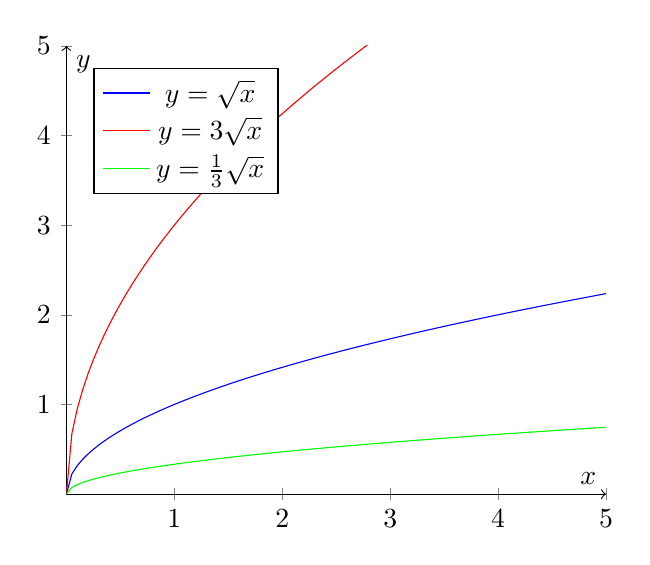
\begin{tikzpicture}
			\begin{axis}[
			  xlabel={$x$},
			  ylabel={$y$},
			  axis lines=middle,
			  axis line style={->},
			  xmin=0,
			  ymin=0,
			  xmax=5,
			  ymax=5,
			  xtick={0,1,2,3,4,5},
			  ytick={0,1,2,3,4,5},
			  xticklabels={0,1,2,3,4,5},
			  yticklabels={0,1,2,3,4,5},
			  legend style={at={(0.05,0.95)},anchor=north west}
			]
			  \addplot[domain=0:5, samples=100, color=blue]{sqrt(x)};
			  \addplot[domain=0:5, samples=100, color=red]{3*sqrt(x)};
			  \addplot[domain=0:5, samples=100, color=green]{(1/3)*sqrt(x)};
			  \legend{$y=\sqrt{x}$, $y=3\sqrt{x}$, $y=\frac{1}{3}\sqrt{x}$}
			\end{axis}
		  \end{tikzpicture}
	\end{align*}
	\item Negative sign results in a reflection. 
	\begin{align*}
		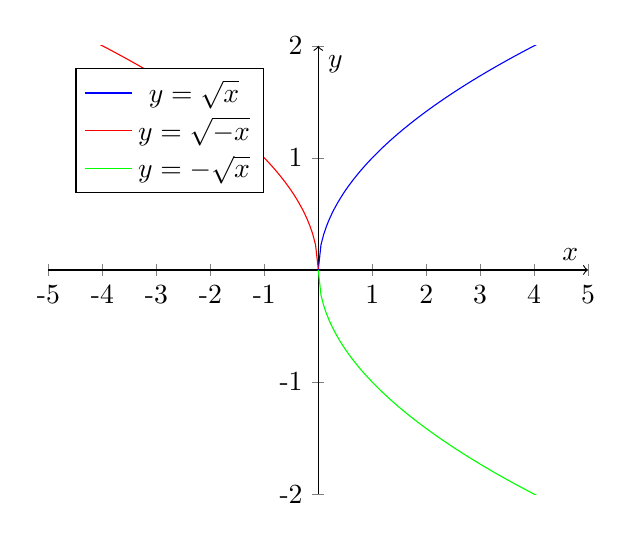
\begin{tikzpicture}
			\begin{axis}[
			  xlabel={$x$},
			  ylabel={$y$},
			  axis lines=middle,
			  axis line style={->},
			  xmin=-5,
			  ymin=-2,
			  xmax=5,
			  ymax=2,
			  xtick={-5,-4,-3,-2,-1,0,1,2,3,4,5},
			  ytick={-2,-1,0,1,2},
			  xticklabels={-5,-4,-3,-2,-1,0,1,2,3,4,5},
			  yticklabels={-2,-1,0,1,2},
			  legend style={at={(0.05,0.95)},anchor=north west}
			]
			  \addplot[domain=0:5, samples=100, color=blue]{sqrt(x)};
			  \addplot[domain=-5:0, samples=100, color=red]{sqrt(-x)};
			  \addplot[domain=0:5, samples=100, color=green]{-sqrt(x)};
			  \legend{$y=\sqrt{x}$, $y=\sqrt{-x}$, $y=-\sqrt{x}$}
			\end{axis}
		  \end{tikzpicture}
	\end{align*}
	As you can see the red graph is the mirror image of the blue graph with respect to the y-axis, and the green graph is the mirror image of the blue graph with respect to the x-axis and also the red graph is the mirror image of the green graph with respect to the x-axis.

\end{itemize}
So whenever we have some operation outside of the function that is going to affect the y-values and whenever we have some operation inside of the function that is going to affect the x-values. \\
When the operation is outside of the function, then it is going to be a shift as we would expect. \\
When the operation is inside of the function, then it is going to be a stretch or compression/shrink the opposite way we'd expect. \\
\subsection{Identifying changes in graphs with respect to another graph}
\textbf{Example.} Consider $y=\sqrt{x}$. How do the graphs of the following functions compare to the graph of $y=\sqrt{x}$  \\

1. $y=\sqrt{x}-4$ \\
\begin{tikzpicture}
	\begin{axis}[
	  xlabel={$x$},
	  ylabel={$y$},
	  axis lines=middle,
	  axis line style={->},
	  xmin=0,
	  ymin=-4,
	  xmax=10,
	  ymax=2,
	  xtick={0,1,2,3,4,5,6,7,8,9,10},
	  ytick={-4,-3,-2,-1,0,1,2},
	  xticklabels={0,1,2,3,4,5,6,7,8,9,10},
	  yticklabels={-4,-3,-2,-1,0,1,2},
	  legend style={at={(0.05,0.95)},anchor=north west}
	]
	  \addplot[domain=0:10, samples=100, color=blue]{sqrt(x)};
	  \addplot[domain=0:10, samples=100, color=red]{sqrt(x) - 4};
	  \legend{$y=\sqrt{x}$, $y=\sqrt{x} - 4$}
	\end{axis}
\end{tikzpicture}
As we can see the graph is shifted down by 4. This is because we subtracted 4 outside of the square root which results in a vertical shift. \\

2. $y=\sqrt{x+12}$ \\
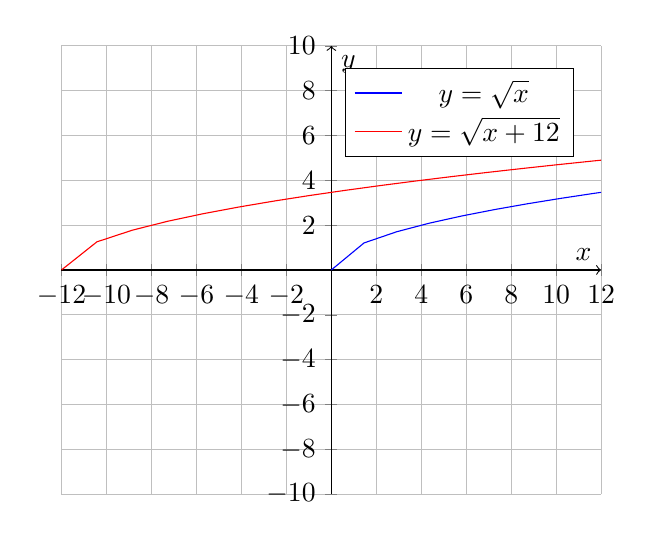
\begin{tikzpicture}
	\begin{axis}[
	  xlabel={$x$},
	  ylabel={$y$},
	  axis lines=middle,
	  axis line style={->},
	  xmin=-12,
	  ymin=-10,
	  xmax=12,
	  ymax=10,
	  xtick={-12,-10,-8,-6,-4,-2,0,2,4,6,8,10,12},
	  ytick={-10,-8,-6,-4,-2,0,2,4,6,8,10},
	  legend style={at={(0.95,0.95)},anchor=north east},
	  grid=both
	]
	  \addplot[domain=0:144, samples=100, color=blue]{sqrt(x)};
	  \addlegendentry{$y=\sqrt{x}$} % Add a legend entry for the first plot
	  % Add a new plot here (shifted 12 units to the left on the x-axis):
	  \addplot[domain=-12:144, samples=100, color=red]{sqrt(x+12)};
	  \addlegendentry{$y=\sqrt{x+12}$} % Add a legend entry for the second plot
	\end{axis}
\end{tikzpicture}
As we can see the graph is shifted to the left by 12. This is because we subtracted 12 inside of the square root which results in a horizontal shift. \\
As we proved before the reason why it is shifted to the left is because the first value that makes sense to the function is -12, because $y=\sqrt{-12+12}=\sqrt{0}=0$. That's where our functions is starting from. \\

3. $y=-3\cdot\sqrt{x}$ \\
Firstly operation outside of the function is going to affect the y-values and since we are multiplying by -3, it is going to strech and since we are introducing a negative sign, it is going to reflect vertically. \\
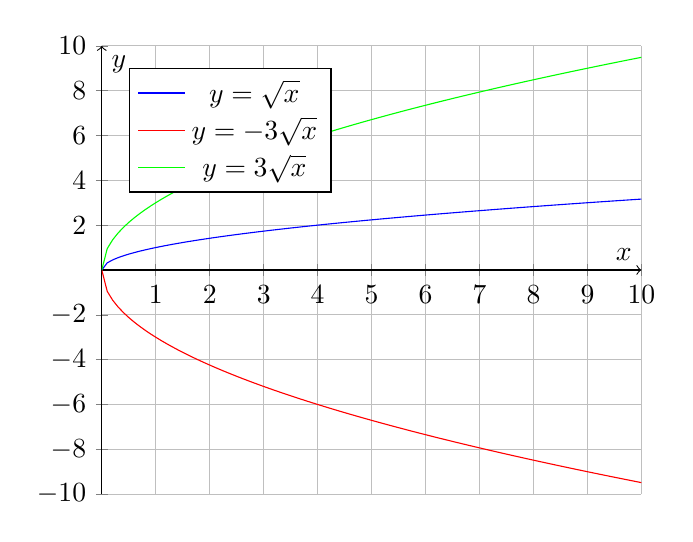
\begin{tikzpicture}
	\begin{axis}[
	  xlabel={$x$},
	  ylabel={$y$},
	  axis lines=middle,
	  axis line style={->},
	  xmin=0,
	  ymin=-10,
	  xmax=10,
	  ymax=10,
	  xtick={0,1,2,3,4,5,6,7,8,9,10},
	  ytick={-10,-8,-6,-4,-2,0,2,4,6,8,10},
	  legend style={at={(0.05,0.95)},anchor=north west},
	  grid=both
	]
	  \addplot[domain=0:10, samples=100, color=blue]{sqrt(x)};
	  \addlegendentry{$y=\sqrt{x}$} % Add a legend entry for the first plot
  
	  \addplot[domain=0:10, samples=100, color=red]{-3*sqrt(x)};
	  \addlegendentry{$y=-3\sqrt{x}$} % Add a legend entry for the second plot
  
	  \addplot[domain=0:10, samples=100, color=green]{3*sqrt(x)};
	  \addlegendentry{$y=3\sqrt{x}$} % Add a legend entry for the third plot
	\end{axis}
  \end{tikzpicture}
We can see that if we would miss the negative sign it would be a stretch and by including it we are reflecting it vertically. \\

4. $y=\sqrt{\frac{1}{4}x}$ \\
Finally we are multiplying by $\frac{1}{4}$ which is going to result in a stretch since it is a multiplication and going to effect the x-values since it is inside of the function. We also know that if it's inside of the function it is going to be the opposite of what we'd expect. So instead of shrinking by $\frac{1}{4}$ it is going to stretch horizontally by 4. \\
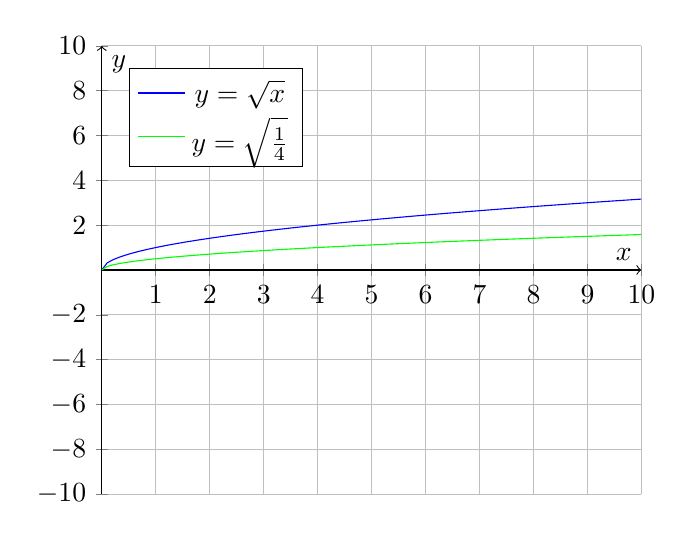
\begin{tikzpicture}
	\begin{axis}[
	  xlabel={$x$},
	  ylabel={$y$},
	  axis lines=middle,
	  axis line style={->},
	  xmin=0,
	  ymin=-10,
	  xmax=10,
	  ymax=10,
	  xtick={0,1,2,3,4,5,6,7,8,9,10},
	  ytick={-10,-8,-6,-4,-2,0,2,4,6,8,10},
	  legend style={at={(0.05,0.95)},anchor=north west},
	  grid=both
	]
	  \addplot[domain=0:10, samples=100, color=blue]{sqrt(x)};
	  \addlegendentry{$y=\sqrt{x}$} % Add a legend entry for the first plot
  
	  \addplot[domain=0:10, samples=100, color=green]{sqrt(0.25*x)};
	  \addlegendentry{$y=\sqrt{\frac{1}{4}}$} % Add a legend entry for the third plot
	\end{axis}
  \end{tikzpicture}

Notice that streching horizontally by 4 looks kind of like shrinking horizontally by a half. 
$$ \sqrt{\frac{1}{4}x} = \sqrt{\frac{1}{4}}\sqrt{x} = \frac{1}{2}\sqrt{x}$$
This proves algebraically that stretching horizontally by 4 is the same as shrinking vertically by a half. \\

\subsubsection*{Summary}
In Summary: \\
\begin{itemize}
	\item Numbers on outside $\Rightarrow$ y-values $\Rightarrow$ vertical shift
	\item Numbers on inside $\Rightarrow$ x-values $\Rightarrow$ horizontal shift
	\item  Adding/Subtraction $\Rightarrow$ shifts
	\item  Multiplication/Division $\Rightarrow$ stretch/shrinks
	\item Negative sign $\Rightarrow$ reflection
\end{itemize} 